\newpage
%\null
%\cleardoublepage



%************************************************************************************************
% Kap.4 Programmentwicklung
%************************************************************************************************

\chapter{Programmentwicklung}
\label{chap:Programmentwicklung}
Bei der Programmentwicklung werden die in Kap. \ref{chap:modellbildung} aufgestellten Gleichungen mit Matlab und Simulink umgesetzt.
Es wird begonnen, die Gleichungen des elektrischen und des mechanischen Teils des Motors, in Simulink umzusetzen.
Im Anschluss folgt die Implementierung der Werte und des Simulinkprogramms des Motors in Matlab.
Daran schliesst sich die Umsetzung der Sensoren in Matlab.
Wenn diese mit Matlabfiles eingebunden werden können, werden die Simulink- und Matlabprogramme des Motors entsprechendn erweitert.

\section{Motor in Simulink}
Es werden die Formeln \ref{equ:motorspannungsimulink} und \ref{equ:motormomentsimulink} aus den Kap. \ref{chap:elekteil} und \ref{chap:mechteil} hergenommen.
Durch ein umstellen der beiden Formeln, so dass nur noch erste Ableitungen in beiden Formeln vorkommen,
lasen sie sich kombinieren und in Simulink einbinden.
Um einen besseren Überblick zu bekommen, werden die Formeln hier noch einmal aufgeführt.
\begin{center}
\begin{equation}
\label{equ:motorspannungsimulink2}
si_A = \frac{1}{L_A} (e_A - R_Ai_A + u_e)
\end{equation}
\end{center}
\begin{center}
\begin{equation}
\label{equ:motorspannungsimulinkkonst2}
e_a = K_M * \phi \omega
\end{equation}
\end{center}
\begin{center}
\begin{equation}
\label{equ:motormomentsimulink2}
s\omega = \frac{1}{J} (M_M - r * \omega - M_L)
\end{equation}
\end{center}
\begin{center}
\begin{equation}
\label{equ:motormomentsimulinkkonst2}
M_M = K_M * \phi *i_A
\end{equation}
\end{center}
$K_M$ und $\phi$ sind Motorkonstanten.

Mit der Annahme das 
\begin{center}
\begin{equation}
\label{equ:variablensimulink}
x_1 := \omega\\
x_2 := i_A
\end{equation}
\end{center}
ist, lässt sich folgendes Gleichungssytem aufstellen:
\begin{center}
\begin{equation}
\label{equ:motormomentsimulink2}
\.x_1 = \frac{1}{J} (K_M \phi x_2 - r * x_1 - M_L)\\
\.x_2 = \frac{1}{L_A} (K_M * \phi x_1 - R_Ax_2 + u_e)
\end{equation}
\end{center}
Dieses Gleichungssytem lässt sich jetzt durch die grafischen Elemente in Simulink sehr einfach modellieren.

Wie zu Begin des Kap. \ref{chap:motor} erwähnt, war es nicht möglich an verschiedenen Werte der Motorkonstanten $K_M$ und $\phi$ zu gelangen.
Aus diesem Grund wird auf die begleitenden Unterlagen der Vorlesung "Systemtechniken" von Prof. Froriep zurück gegriffen.

Auf dieser Grundlage werden die weiteren Programme entwickelt.

Um eine Regelung aufzubauen, wird noch ein Regler, ein Sollwertgeber und ein Subtrahierer von Ist- und Sollwert benötigt.
Diese werden über die Simulinkbibliothek eingebunden und entsprechende Verbindungen angelegt.
Das fertige Grundprogramm ist in Abb. \ref{fig:grundprogramm} dargestellt.
\begin{figure}[!h]
	\centering
	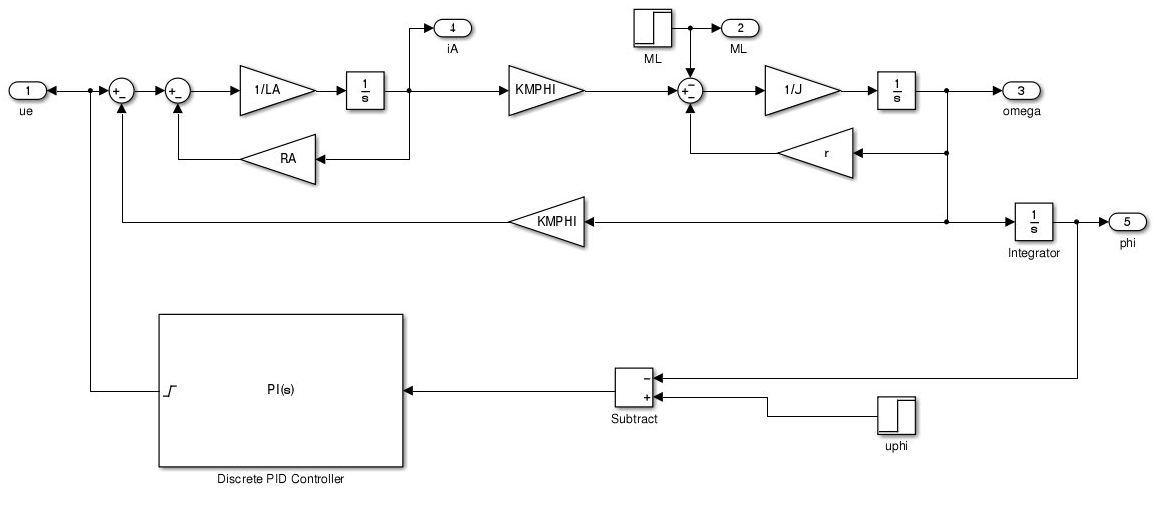
\includegraphics[width=0.6\textwidth]{sSpiegel.jpg}
	\caption{Simulink Grundprogramm}
	\label{fig:grundprogramm}
\end{figure}

\section{Matlab}
\subsection{Motor in Matlab}
Die Programmentwicklung in Matlab gestaltet sich für den Motor als relativ einfach, da, wie oben erwähnt, keien Motordaten gefunden wurden, wird auf das Matlabfile von 
Prof. Froriep aus der Vorlesung "Systemtechniken" zurück gegriffen.
In diesem Matlabfile stehen die Motorkenndaten, die berechnete Trägheit des Spiegels, das berechnete Drehmoment, die Grenzen für die Plots, Anweisungen für die Plots und
für den Integrationsalgorithmus.
Dieses File ist eine sehr gute Grundlage für die Simuation, welches während der Simulation entsprechend angepasst werden kann.

\subsection{Sensor in Matlab}
